\section{Results}\label{sec:results}
In this section, we describe the results of our experiment. 

\begin{figure*}[t!]
    \centering
    \subfigure[North American resolvers]{%
        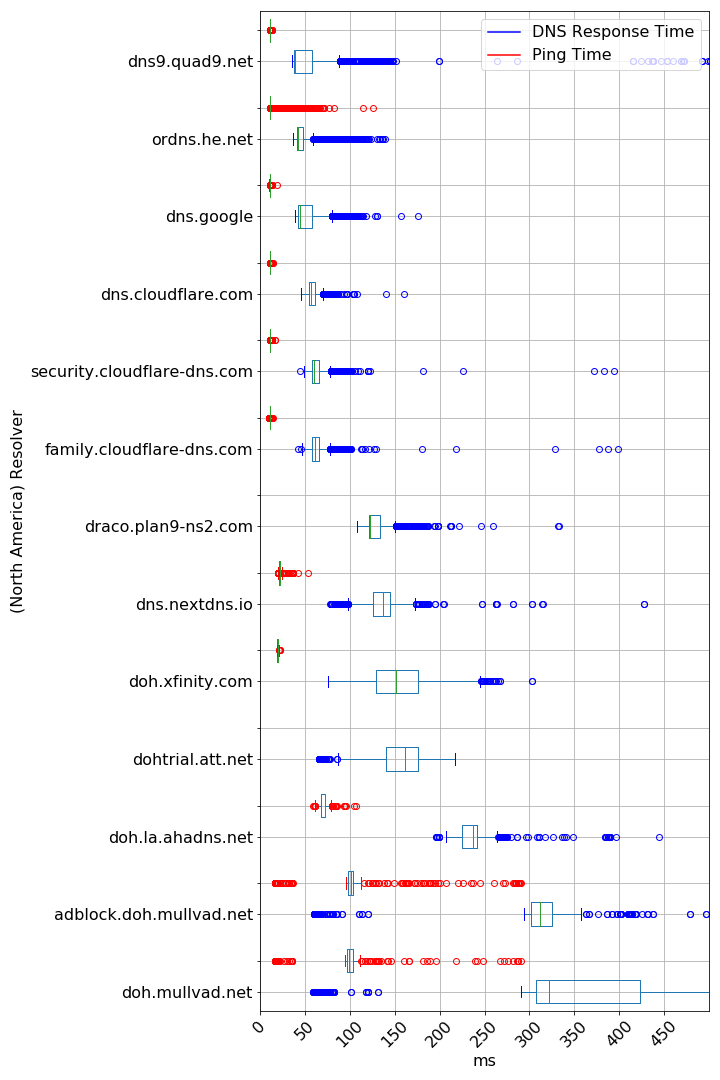
\includegraphics[width=0.5\textwidth]{figures/Ohio_North_America.png}
    }
    \subfigure[Asian resolvers]{%
        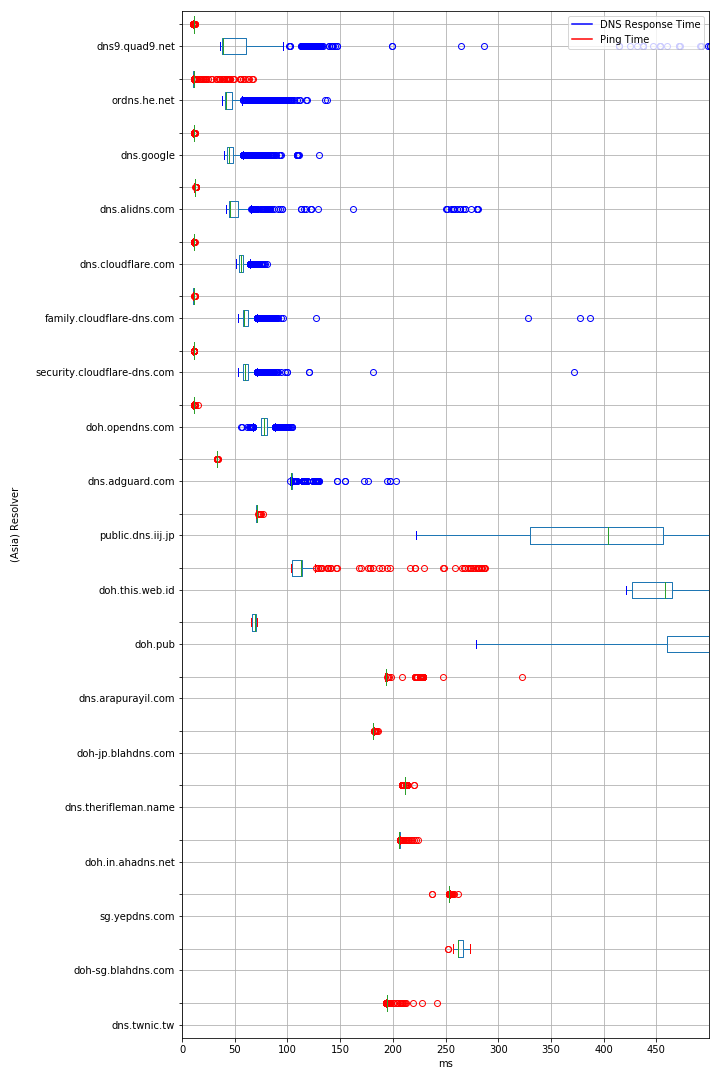
\includegraphics[width=0.5\textwidth]{figures/Ohio_Asia.png}
    }
    \subfigure[European resolvers]{%
        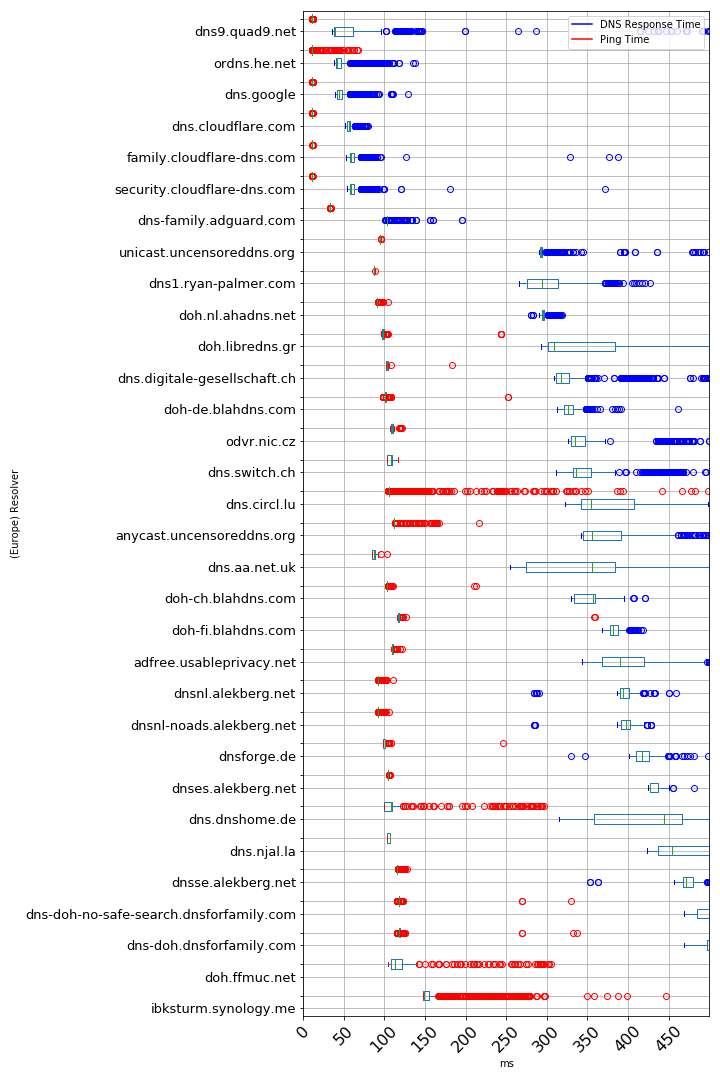
\includegraphics[width=0.5\textwidth]{figures/Ohio_Europe.png}
    }
    \caption{Box-plots of resolvers measured from a vantage point in Ohio, USA}
\end{figure*}

\begin{figure*}[t!]
    \centering
    \subfigure[North American resolvers]{%
        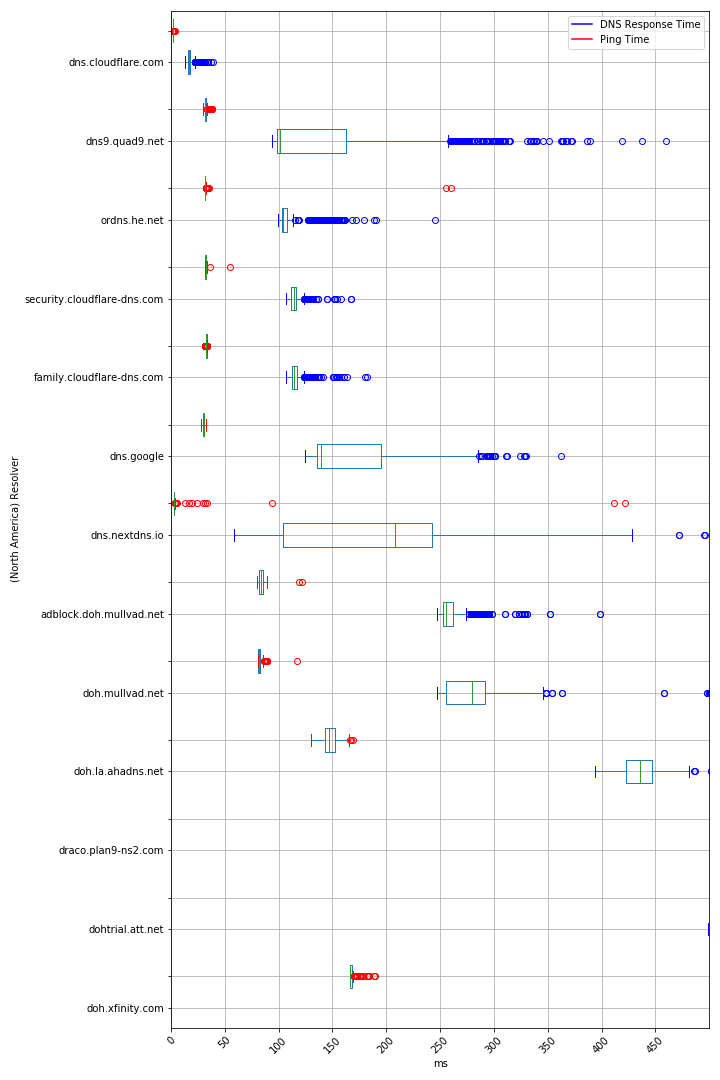
\includegraphics[width=0.5\textwidth]{figures/Seoul_North_America.png}
    }
    \subfigure[Asian resolvers]{%
        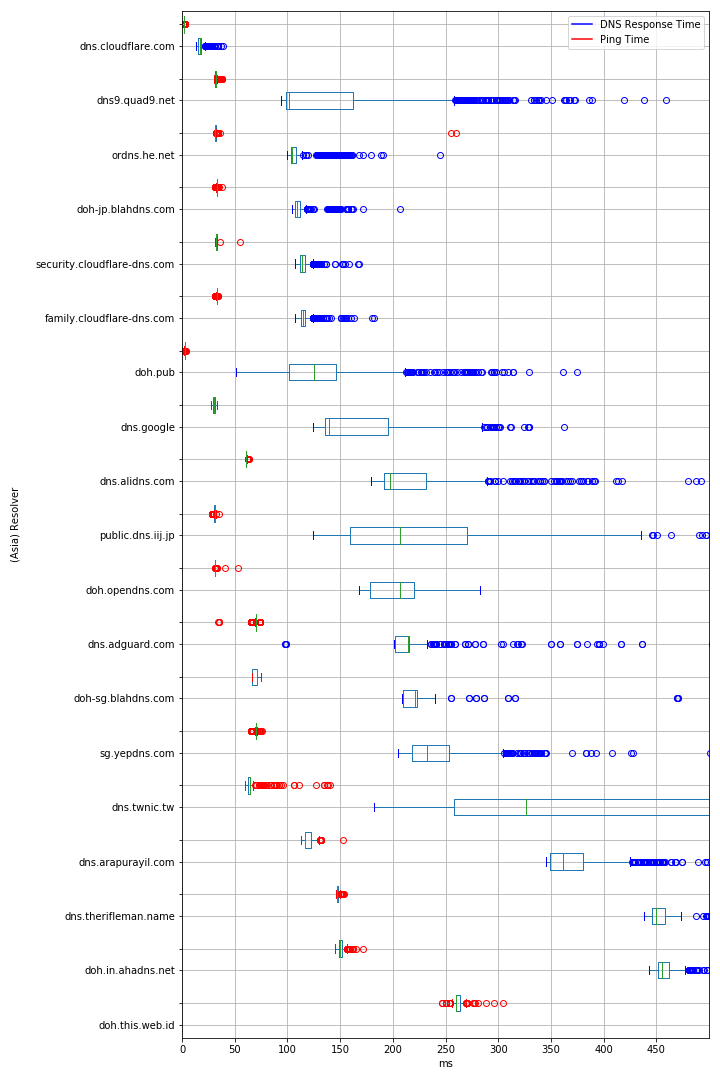
\includegraphics[width=0.5\textwidth]{figures/Seoul_Asia.png}
    }
    \subfigure[European resolvers]{%
        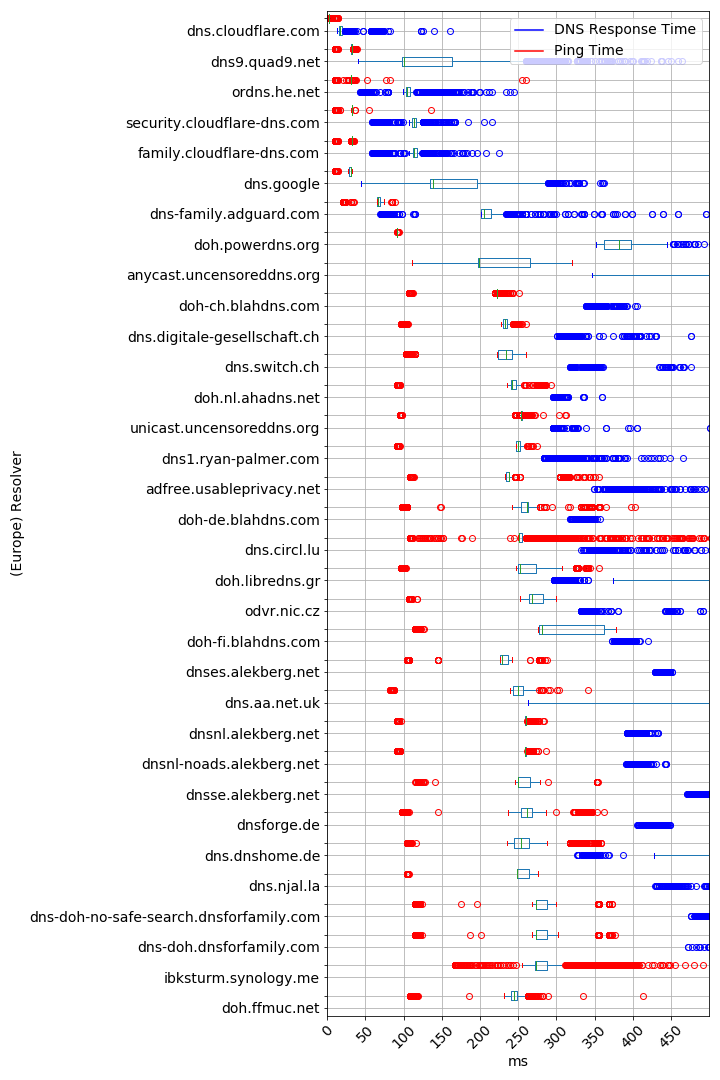
\includegraphics[width=0.5\textwidth]{figures/Seoul_Europe.png}
    }
    \caption{Box-plots of resolvers measured from a vantage point in Seoul, South Korea}
\end{figure*}

\begin{figure*}[t!]
    \centering
    \subfigure[North American resolvers]{%
        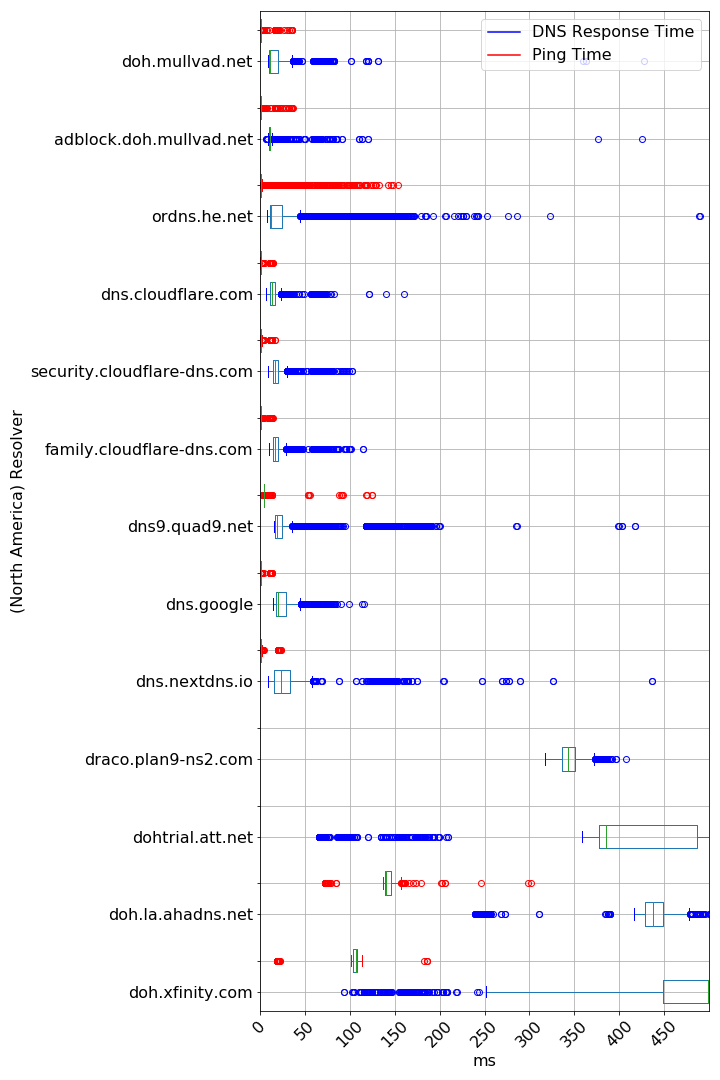
\includegraphics[width=0.5\textwidth]{figures/Frankfurt_North_America.png}
    }
    \subfigure[Asian resolvers]{%
        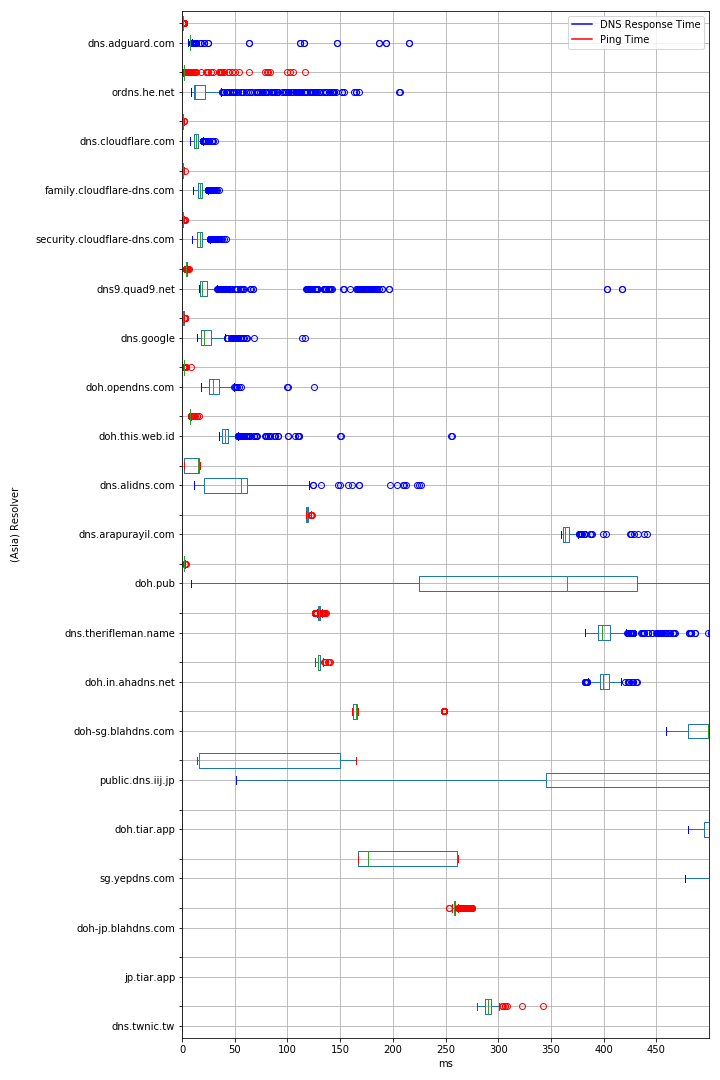
\includegraphics[width=0.5\textwidth]{figures/Frankfurt_Asia.png}
    }
    \subfigure[European resolvers]{%
        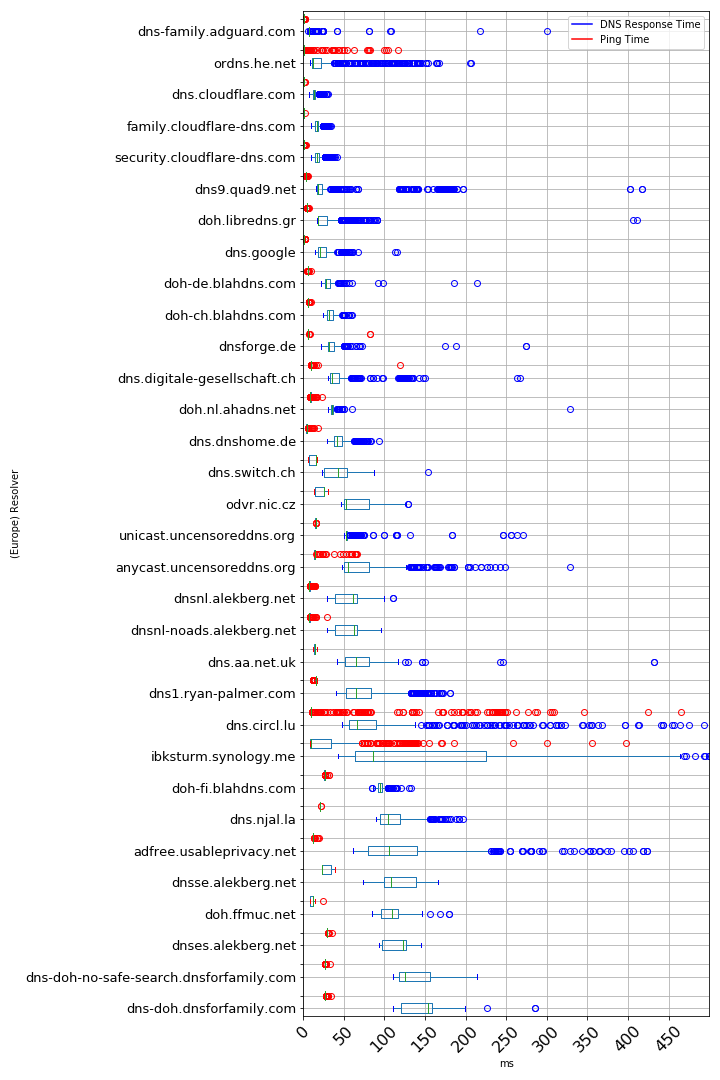
\includegraphics[width=0.5\textwidth]{figures/Frankfurt_Europe.png}
    }
    \caption{Box-plots of resolvers measured from a vantage point in Frankfurt, Germany}
\end{figure*}

\begin{figure*}[t!]
    \centering
    \subfigure[North American resolvers]{%
        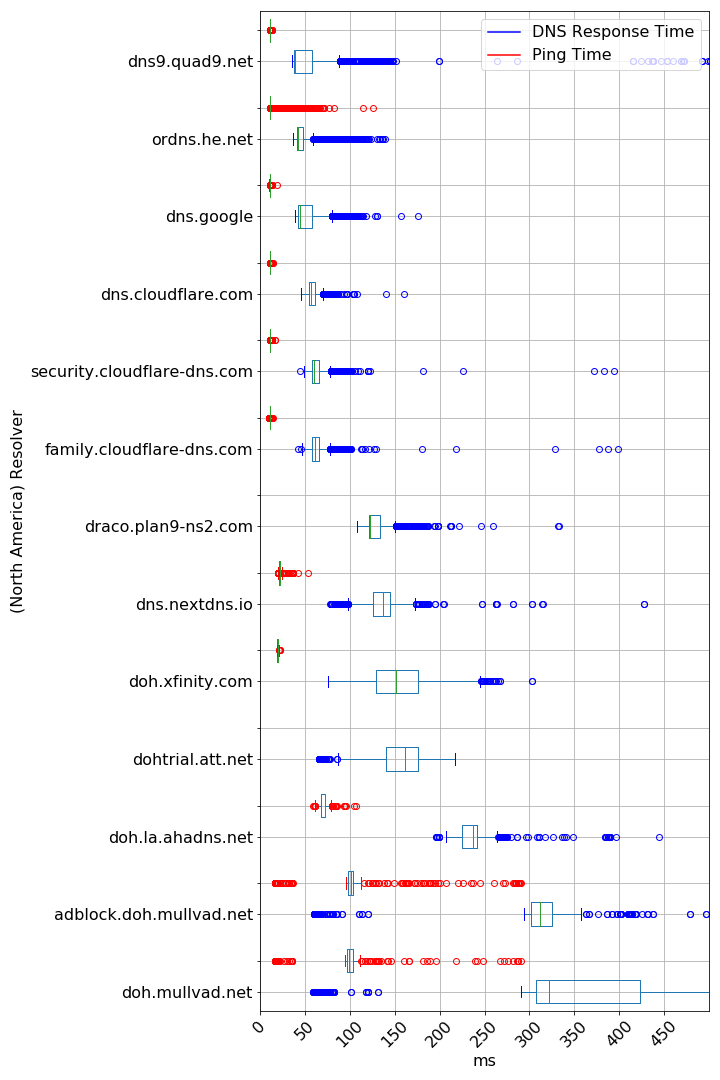
\includegraphics[width=0.5\textwidth]{figures/Ohio_North_America.png}
    }
    \subfigure[Asian resolvers]{%
        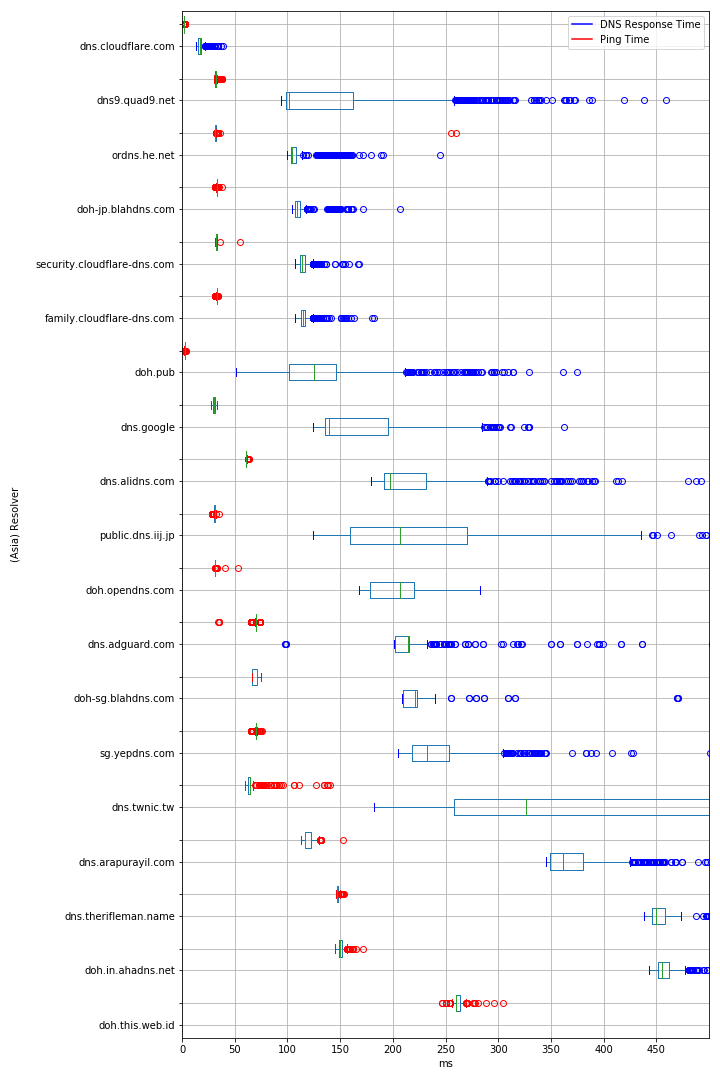
\includegraphics[width=0.5\textwidth]{figures/Seoul_Asia.png}
    }
    \subfigure[European resolvers]{%
        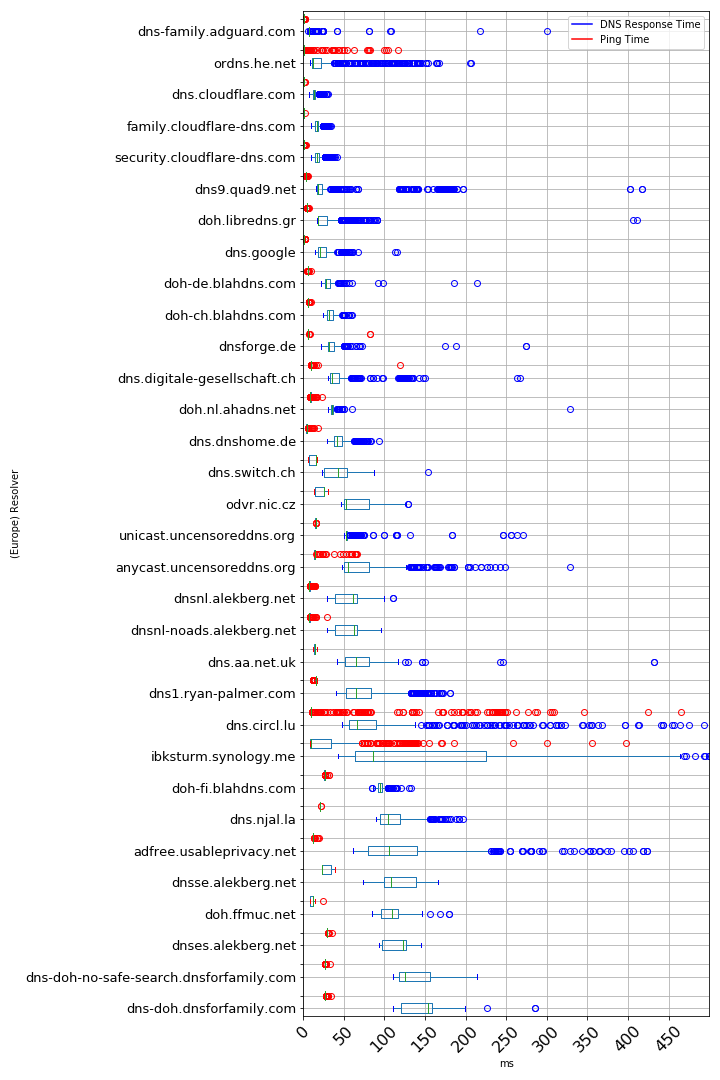
\includegraphics[width=0.5\textwidth]{figures/Frankfurt_Europe.png}
    }
    \caption{Comparing local to local}
\end{figure*}

\begin{table}[]
\begin{tabular}{|l|l|}
\hline
\textbf{Location} & \textbf{Resolver}                                                                                                                     \\ \hline
North America     & \begin{tabular}[c]{@{}l@{}}dnscrypt.ca-1-doh\\ dnscrypt.ca-2-doh\\ doh-cleanbrowsing\\ pf-doh\end{tabular}                            \\ \hline
Asia              & \begin{tabular}[c]{@{}l@{}}dns.arapurayil-doh-in\\ doh.tiarap.org\\ jp.tiarap.org\\ doh.linuxsec\\ sg.yepdns\end{tabular}             \\ \hline
Europe            & \begin{tabular}[c]{@{}l@{}}dnsnl-noads.alekberg\\ doh.bortzmeyer\\ doh.appliedprivacy\\ meganerd-doh-ipv4\\ doh.powerdns\end{tabular} \\ \hline
\end{tabular}
\caption{Resolvers that failed to respond}
\label{table:UnresponsiveResolvers}
\end{table}

% Please add the following required packages to your document preamble:
% \usepackage[normalem]{ulem}
% \useunder{\uline}{\ul}{}
\begin{table}[]
\begin{tabular}{lll}
\hline
\textbf{Resolver}  & \textbf{DNS Response Time (ms) from Seoul Vantage Point} & 
\textbf{DNS Response Time (ms) from Ohio Vantage Point}  \\ \hline
doh-jp.blahdns.com & 109.41                                                   & 601.61                                          \\ \hline
doh.in.ahadns.net  & 454.93                                                   & 643.88                                          \\ \hline
dns.twnic.tw       & 326.19                                                   & 1573.37                                         \\ \hline
sg.yepdns.com      & 232.69                                                   & 707.05                                          \\ \hline
\end{tabular}
\caption{Performance of non-conventional resolvers located in Asia}
\label{table:UnconvAsia}
\end{table}

% Please add the following required packages to your document preamble:
% \usepackage[normalem]{ulem}
% \useunder{\uline}{\ul}{}
\begin{table}[]
\begin{tabular}{lll}
\hline
\textbf{Resolver}    & \textbf{DNS Response Time (ms) from Frankfurt Vantage Point} & \textbf{DNS Response Time (ms) from Seoul Vantage Point} \\ \hline
doh.libredns.gr      & 18.89                                                        & 803.67                                          \\ \hline
doh.nl.ahadns.net    & 36.11                                                        & 778.35                                          \\ \hline
dns.dnshome.de       & 42.28                                                        & 1041.77                                         \\ \hline
dns1.ryan-palmer.com & 65.43                                                        & 779.27                                          \\ \hline
\end{tabular}
\caption{Performance of non-conventional resolvers located in Europe}
\label{table:UnconvEur}
\end{table}


\subsection{How do Mainstream Resolvers Compare to Non-Mainstream Resolvers}


\subsection{Does Network Distance Correlate to Response Times?}

We find that certain conventional resolvers including \texttt{dns.google} and \texttt{dns9.quad9}, except for \texttt{dns.cloudflare} which actually performs better, have higher response times in Seoul than in Ohio. 
However, as Table ~\ref{table:UnconvAsia} indicates, non-conventional resolvers located in Asia perform better from the Seoul vantage point than the Ohio vantage point. 
Similarly, Table ~\ref{table:UnconvEur} demonstrates that the response times of European non-conventional resolvers measured from Frankfurt is much lower than the response times of those same resolvers measured from Seoul. 
We find a correlation between network distance and response times. 




















